\chapter{Descrição do sistema de controle}

O presente trabalho busca controlar a posição de um carro ao longo de uma guia linear. Para realizar essa tarefa, foi escolhida a realimentação de estados como estratégia de controle.

\section{Projeto Realimentação de Estados}

Na realimentação de estados, são determinados requisitos para o sistema, de tal forma que esses correspondem a novos polos do sistema no plano complexo; para tal, uma lei de controle para a mudança dos polos é estabelecida, em que $U(t) = KX(t)$ é o vetor de controle, onde $K \in \mathbb{R}^{n_u \times n}$. A Figura \ref{fig:diagrama_blocos} apresenta o diagrama de blocos com a presença do controlador via realimentação de estados.

\begin{figure}[H]
    \centering
    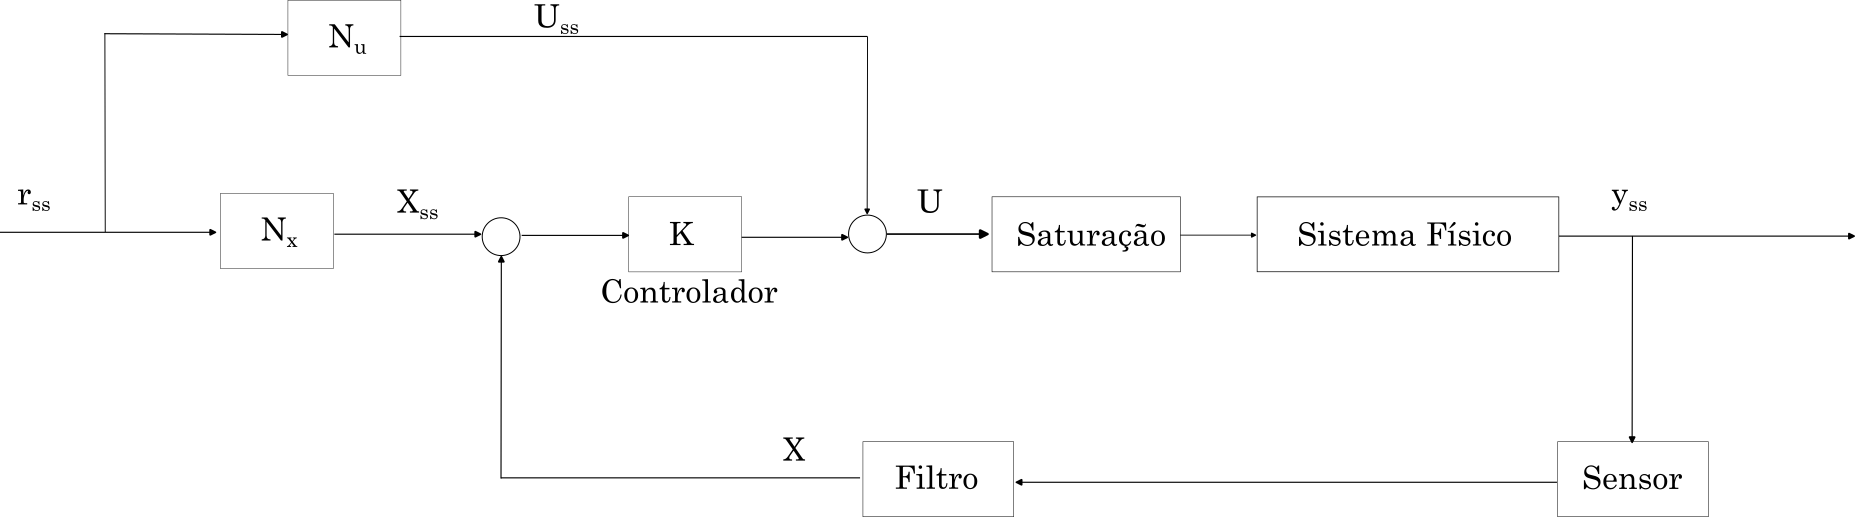
\includegraphics[width=1\linewidth]{figuras/diagrama_blocos.png}
    \caption[Diagrama de blocos da planta]{Diagrama de blocos da planta.}
    \label{fig:diagrama_blocos}
\end{figure}

Conforme mostrado na Figura \ref{fig:diagrama_blocos}, o sistema possui limitações físicas, dessa forma a variável de controle (u) está sujeita a saturação. No caso do sistema estabelecido, a variável de controle é a tensão aplicada no motor CC, medida em Volts, podendo ser na faixa de -12 V a +12 V.

A saída do sensor é submetida ao filtro abordado no Apêndice \ref{apend:1}. A referência ($r_{ss}$) se torna a nova entrada da planta, sendo submetida aos ganhos $N_x$ e $N_u$. A entrada do controlador se torna a diferença entre a referência e a saída atual (y).

\section{Espaço de Estados a tempo discreto}

